% This is samplepaper.tex, a sample chapter demonstrating the
% LLNCS macro package for Springer Computer Science proceedings;
% Version 2.20 of 2017/10/04
%
\documentclass[runningheads]{llncs}
%
\usepackage{graphicx}
\usepackage{rotating}
% Used for displaying a sample figure. If possible, figure files should
% be included in EPS format.
\usepackage[english]{babel}
\usepackage[utf8]{inputenc}
\usepackage{amsmath}
\usepackage{csquotes}% Recommended
\usepackage{pgfgantt}

\usepackage[style=authoryear-ibid,backend=biber]{biblatex}

\addbibresource{ref.bib}% Syntax for version >= 1.2
%
% If you use the hyperref package, please uncomment the following line
% to display URLs in blue roman font according to Springer's eBook style:
% \renewcommand\UrlFont{\color{blue}\rmfamily}

\begin{document}
%
\title{A computer-vision based training coach for computerized physical training}
%
%\titlerunning{Abbreviated paper title}
% If the paper title is too long for the running head, you can set
% an abbreviated paper title here
%
\author{George Davies\orcidID{0009-0008-4132-5676}}
%
\authorrunning{G. Davies}
% First names are abbreviated in the running head.
% If there are more than two authors, 'et al.' is used.
%
\institute{University of Lincoln, UK 
\email{27421138@students.lincoln.ac.uk}}
%
\maketitle              % typeset the header of the contribution
%

% The project proposal should be aligned with your programme of study and be produced following discussions with your supervisor around the suitability and scope of the research you will undertake. The work you will do for the proposal will help you frame the independent research you will do for the module's duration. As with all assessments for the module, you will be expected to undertake research yourself and make informed decisions independently that support your project’s research aims and objectives. The recommended structure for the proposal document can be found under the “Additional Information” section of this briefing document. Your submission should conform to one of the suppled templates and be submitted as a PDF as per school policy. The templates can be downloaded from Blackboard under Assessments>Assessment Documents>Assessment Item 1.

% Ethical approval (where applicable)
% If your project is likely to involve human participants in a low-risk capacity (e.g., a user study) then you must complete an ethics application via LEAS. Your LEAS application must be submitted to the LEAS service by the same deadline as the proposal. You should discuss this with your supervisor before completing your ethics application, your supervisor will provide support for this. Consideration of ethical issues must also be evidenced in the ‘Ethical Considerations’ section of the project proposal.

\section{Introduction} % ~700 words
    In many stories of science-fiction, there are robots that are intelligent, borderline human in the way they talk, the way they walk, and the way they interact with their environments. These kinds of robots seem to be creatures that won't exist any time soon, and they probably won't, but with every advancement in the field of robotics and autonomous systems, we step closer to that reality. One key sense that helps a robot communicate and understand its environment is sight, and the area of robotics that strives towards the goal of giving machines the sense of sight is computer vision. 

    \subsection{Area of Research}
        Human Pose Estimation (HPE) is an area of research within computer vision that aims to teach robots how to make sense of the human form and the motions it is capable of performing. It involves the identification and classification of the joints in the human body, capturing a set of coordinates for each joint, known as a key point, that can describe the pose of a person. HPE has a wide set of uses in many fields: In games, with motion capture technologies reliant on HPE, it allows developers to code program more realistic and fluid character movements. In healthcare, healthcare providers can monitor a patient's movements and detect any abnormalities. Augmented reality, allows the user to interact with the digital content in more natural and intuitive ways with gestures. And finally, the use-case that is the primary focus of this project, is sports training. HPE can be used to analyse a user's performance, identify areas for improvement, and develop personalised training programs based on the physical level of the user. For example, HPE could be used to analyse a runner's form, e.g. How straight is their back? What part of the foot are they landing on? Are they leaning more to one side?..., and provide feedback on how to improve their technique. HPE can be used to collect data about any exercises where the movement of the body is vital to its effectiveness.
    
    \subsection{Relevance to the Degree Programme}
        I am enrolled in the MSc programme Robotics and Autonomous Systems at the Univerity of Lincoln through the AgriFoRwArdS CDT.\@ Throughout the first two semesters, I studied the principles of robotics, artificial intelligence, machine learning, and computer vision. Principles from all of these subjects are applied within the area of research on human pose estimation. As to my affiliation with the AgriFoRwArdS CDT, their focus is on the production and use of AI, ML, and CV applications to help the farming and agricultural industries, as Lincolnshire is an agricultural region of the UK.\@ Human pose estimation has previously been used in agritech applications \parencite{app12168160}, with its ability to facilitate human-robot interactions in the field for fruit picking, robotic carts will follow the worker through the field to hold the produce and take it away once full. HPE allows these robots to understand gesture commands the worker may give it, and gives the robot an understanding of humans that allows it to find and follow them without driving into them.
        


    \subsection{Background of the Topic}
        When computer vision gained popularity in the late 1960s and early 1970s, HPE research had its start. Scientists first focused on basic problems like as shape analysis, object recognition, and visual understanding. As computer vision developed, HPE became a stand-alone area of study \parencite{Roboflow}. Historically, HPE was frequently described probabilistically to account for likely inference ambiguities. Since deep learning has been more widely used, the focus has switched to end-to-end trainable models because of their ability to extract intricate patterns and postures from data. Traditionally, computer vision systems have assessed an object's or person's posture by geometric calculations and feature-based techniques. But, the biggest developments in HPE came with the advent of deep neural networks, convolutional neural networks, and computer vision. The field has advanced considerably in spite of these challenges, and more recent techniques that make use of properly designed neural networks may provide amazing results in challenging scenarios involving a large number of, perhaps veiled, interacting individuals \parencite{liu2018recognizing}. Now that these detections have the necessary technology and are sufficiently precise, they may be employed for commercial purposes. It also offers a wealth of new application potential and signifies a major change in HPE's overall direction.



\section{Aims and Objectives} % ~300 words
%You should formulate these clearly, explaining what problems are to be explored and why they are worth exploring. You should have a single overarching aim that comprises your overall research question.
    \subsection{Aims}
        
        \begin{itemize}
            \item Specific: The goal of this project is to create an AI fitness personal trainer application capable of using video input to detect the presence of the user, finding and identifying the keypoints on the user's body, analysing the poses created by the connections between the keypoints (while making inferences on the position of occluded keypoints), and of giving the user recommendations on how to improve the user's form to help minimise the risk of injury and maximise the effectiveness of the chosen exercise. If there is time, a potential add-on would be to make this a smartphone application for ease of use.
            \item Mesurable: The success of this application can be measured by its ability to detect certain movements. First by its ability to detect the human shape then the exercises and the form.
            \item Achievable: This task is certainly acheivable, I have previous experience with image processing using python.
            \item Relavant: This project is worthwhile for many reasons, a few of them I describe in section 2.3. below.
            \item Timebound: The deadline for this research project is currently set to the 29th of August 2024. Giving a two month timeframe to complete the project.
        \end{itemize}    

    \subsection{Issues to Explore}
        There are many issues relating to the subject of human pose estimation. Namely, how to detect keypoints on the human body more efficiently to allow for real-time detection and processing. How to effectively infer the positions of keypoints occluded by other body parts or obstacles. And how to use the data to derive recommendations on how to improve the user's form.

    \subsection{Motivation}
        Over the last few decades, the percentage of people who are either overweight or obese has steadily increased. This is a concerning trend as being obese increases the risk of many other health conditions such as type 2 diabetes, coronary heart disease, some types of cancer, and stroke \parencite{NHS-obesity}. As seen in Figure~\ref{fig:obesity}, over 60\% of the UK population is considered overweight or obese. \\

        \begin{figure}[htbp]
            \centering
            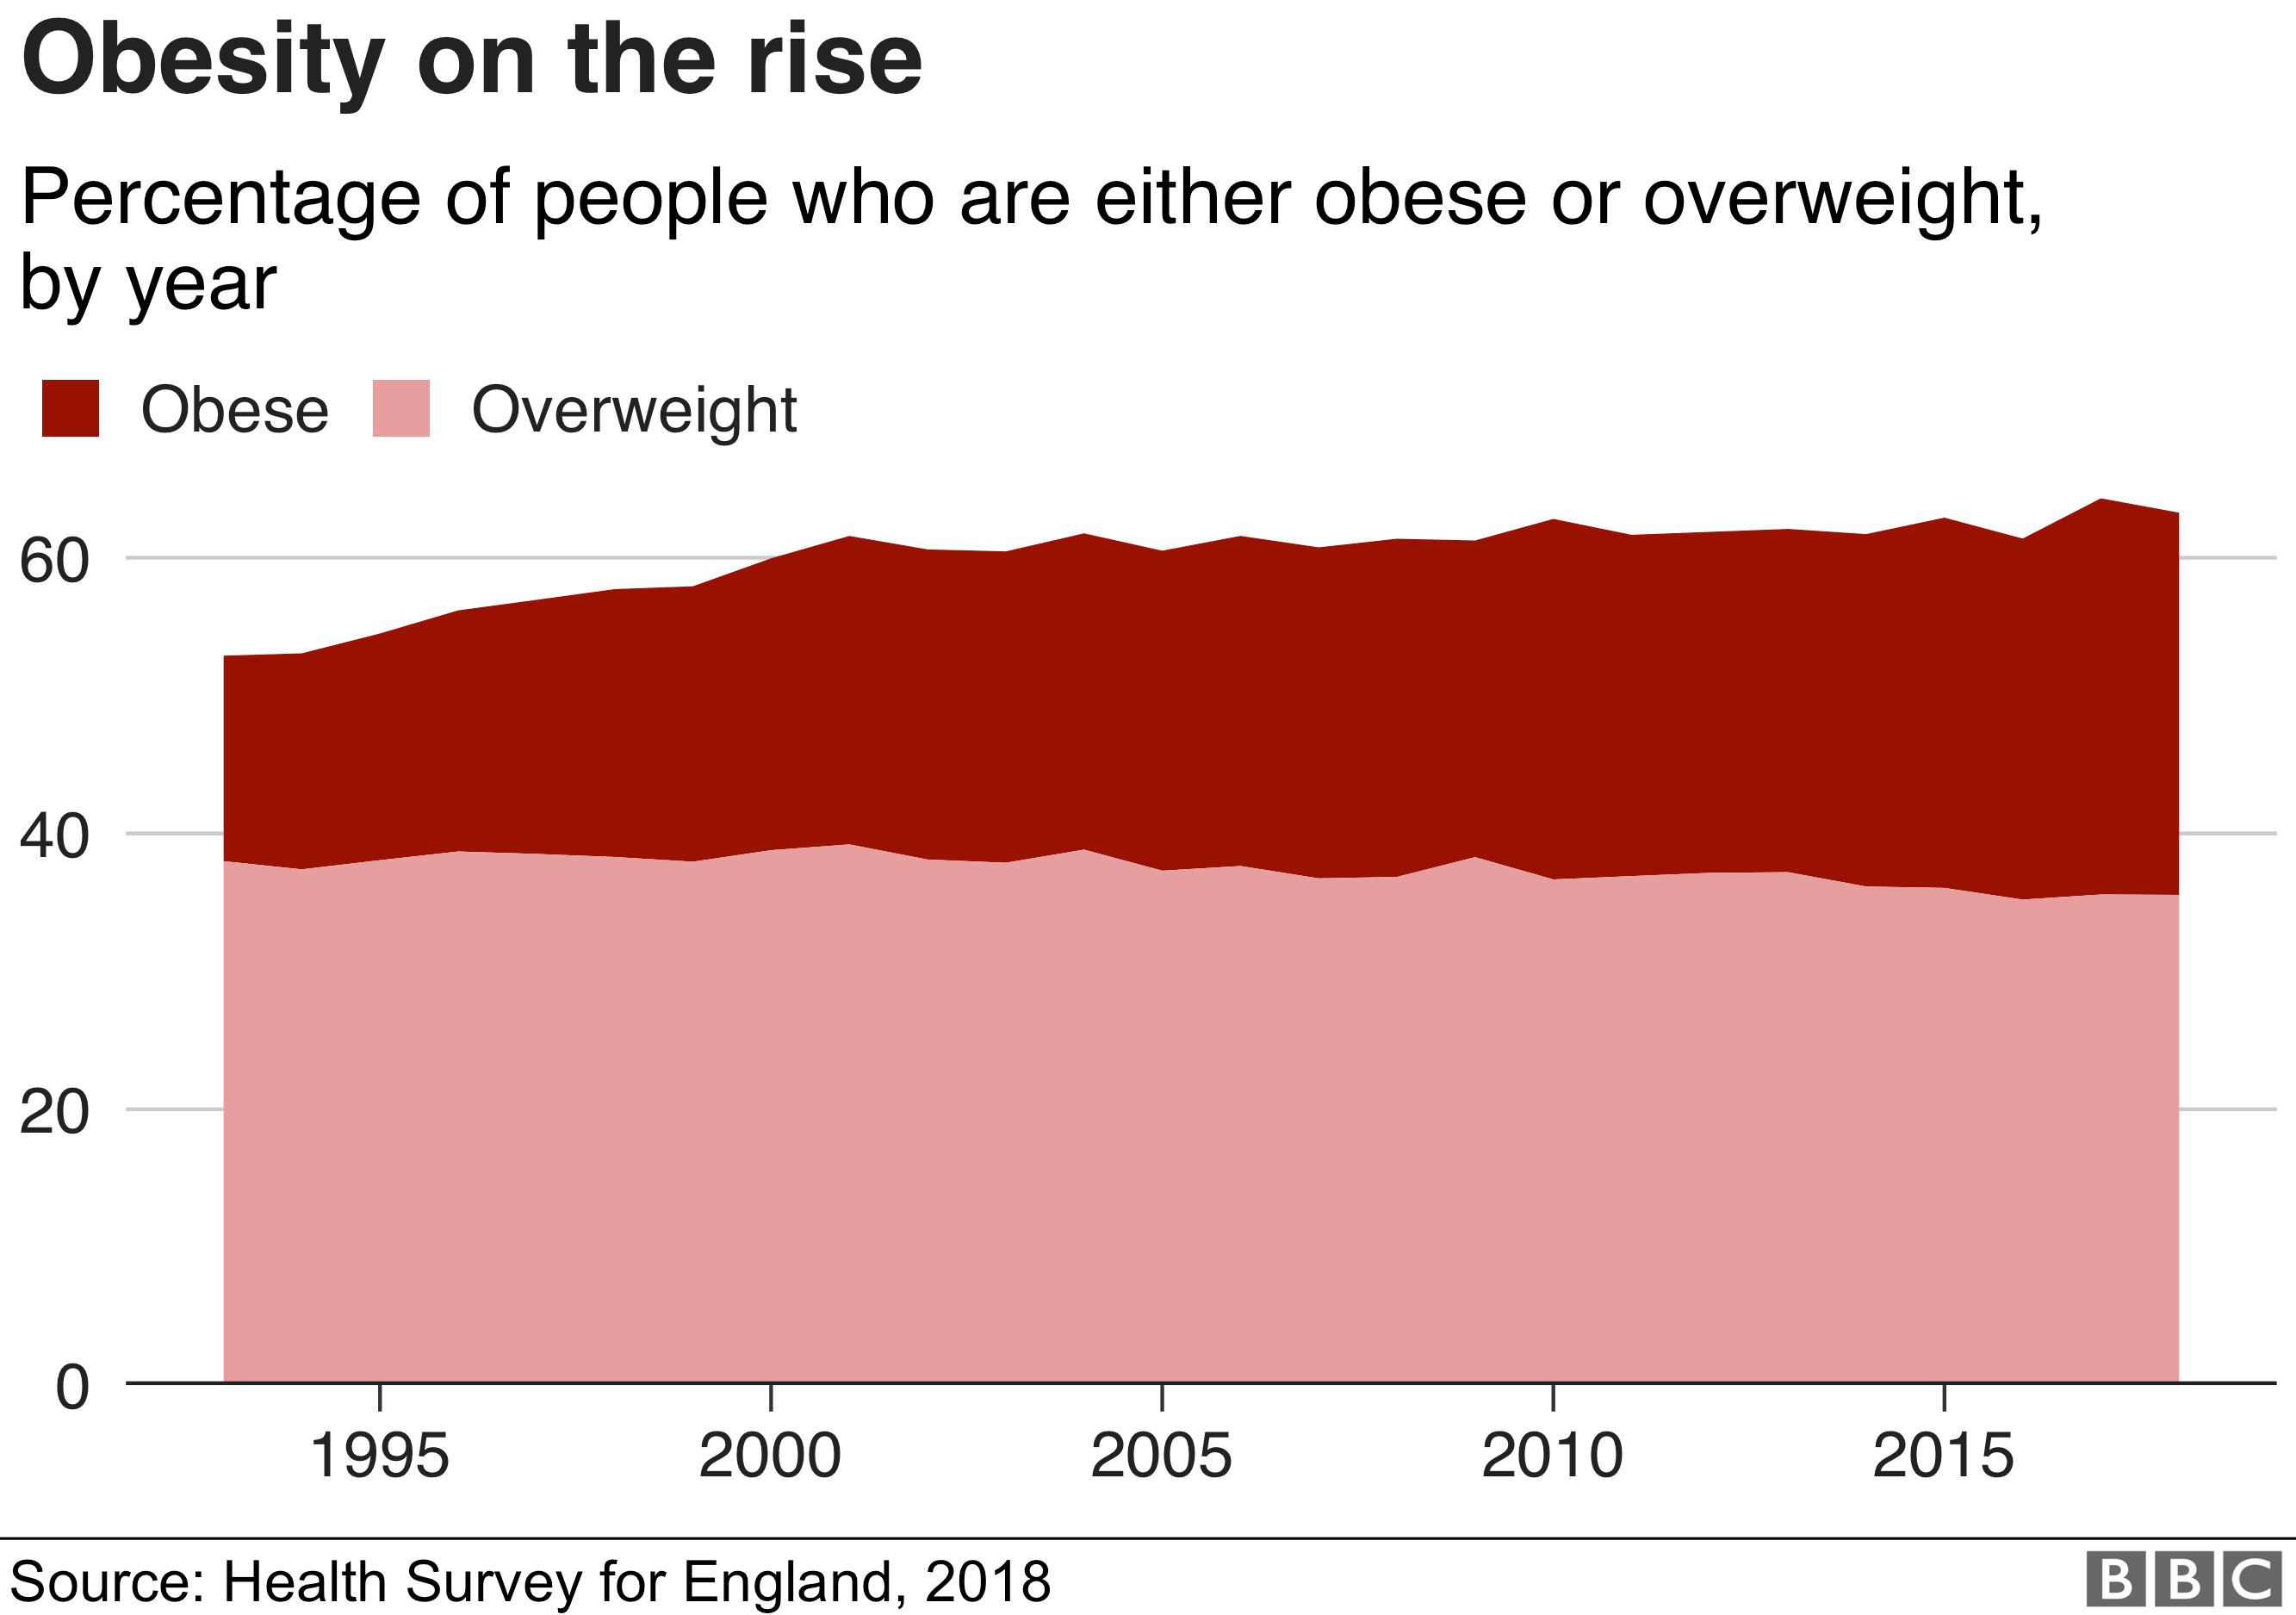
\includegraphics[width=0.33\textwidth]{figures/obesity.png}
            \caption{Percentage of people who are either obses or overweight, by year (Source: Health Survey for England, 2018)}\label{fig:obesity}
        \end{figure}

        To help solve that issue, it is important to encourage people to workout, but going to the gym can be daunting, especially when you don't know how to perform exercises properly. Creating an AI personal trainer will give people the knowledge and confidence to exercise more at home or the gym. Furthermore, exercise has many benefits other than weight loss, it reduces the risk of the issues mentioned above and has been shown to improve mental health \parencite{NHS-benefits}.

    


\section{Literature Survey} % ~700 words
%Provide a short literature survey based on key pieces of work. For example, 3 or 4 relevant papers on the topic of interest will suffice.

    \subsection{BlazePose: On-device Real-time Body Pose tracking \parencite{bazarevsky2020blazeposeondevicerealtimebody}}
        This 2020 Google Research by Valentin Bazarevsky et al.\@ demonstrates a particular type of convolutional neural network architecture called BlazePose which was created specifically for the real-time mobile human posture estimation task. 
        With the ability to build 33 body keypoints for an individual and operating at over 30 frames per second on a Pixel 2, it is perfect for real-time applications such as fitness tracking and sign language recognition. BlazePose's primary contributions are a lightweight body pose estimate neural network and a novel body pose tracking method. 
        Regression and heatmaps are both used by the network to determine keypoint coordinates, which probably improves efficiency and accuracy. An important development in the realm of on-device real-time body posture monitoring is this technology. It is a useful instrument for a variety of applications due to its efficiency and adaptability. BlazePose has a bright future ahead of it, and it will be interesting to watch how this technology develops and is applied in many real-world scenarios.
        \begin{figure}[htbp]
            \centering
            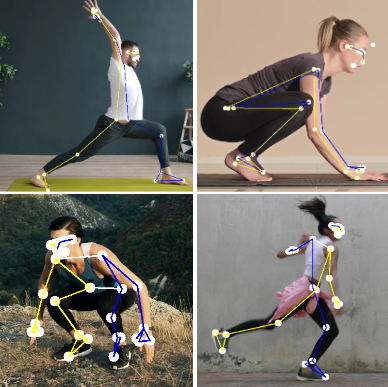
\includegraphics[width=0.33\textwidth]{figures/BlazePose.png}
            \caption{BlazePose results on yoga and fitness poses}
        \end{figure}

    \subsection{Realtime Multi-Person 2D Pose Estimation using Part Affinity Fields \parencite{cao2017realtimemultiperson2dpose}}
        In this 2017 paper by Zhe Cao et al., an effective technique for predicting posture for several people is Real-Time Multi-Person 2D posture estimate using Part Affinity Fields (PAFs) is presented. This method seeks to identify several individuals' 2D postures inside a picture. The system gains the ability to link body parts with specific persons in the image by using a nonparametric representation called Part Affinity Fields (PAFs). PAFs, or groups of 2D vector fields, represent the limbs' orientation and posture inside an image. Regardless of the number of persons in the image, the system's architecture for a greedy bottom-up parsing phase that produces exceptional accuracy and real-time speed.\\

        \begin{figure}[htbp]
            \centering
            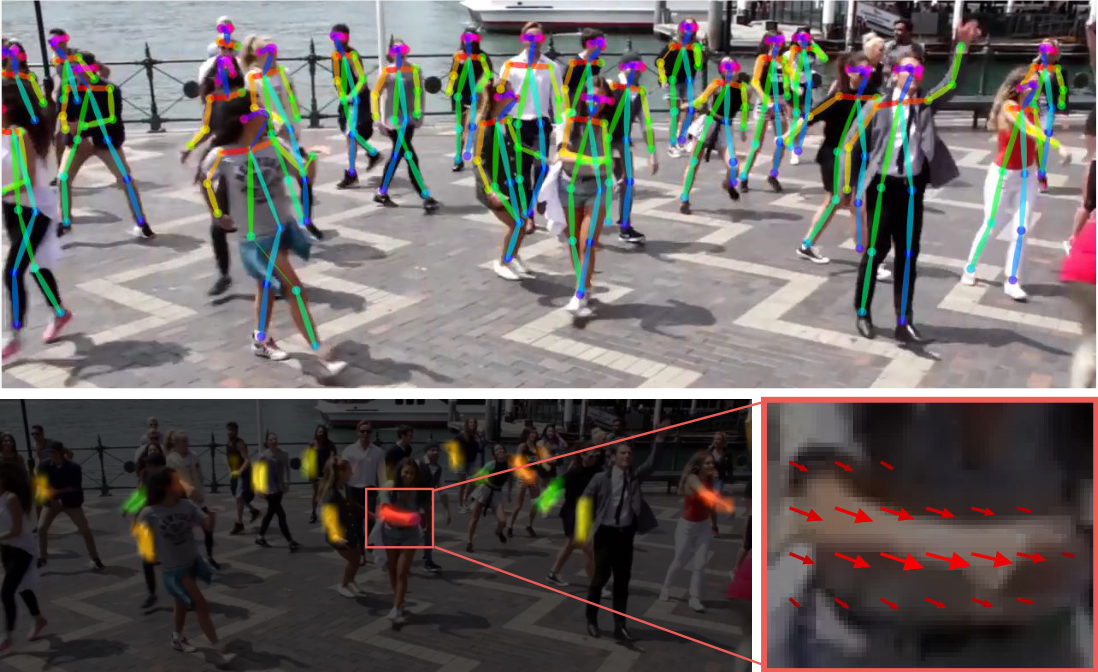
\includegraphics[width=0.5\textwidth]{figures/multipose.png}
            \caption{Top: Multi-person pose estimation. Body parts belonging to the same person are linked. Bottom left: Part Affinity Fields (PAFs) corresponding to the limb connecting right elbow and right wrist. The color encodes orientation. Bottom right: A zoomed in view of the predicted PAFs. At each pixel in the field, a 2D vector encodes the position and orientation of the limbs.}
        \end{figure}

        It is therefore especially appropriate for use cases that include real-time data. The main contribution of this strategy is the separation of image population and runtime complexity. Compared to previous methods, which often saw increased computational costs as the number of participants increased, this represents a significant breakthrough. In summary, real-time multi-person 2D posture estimation using Part Affinity Fields presents this innovative and efficient approach for multi-person posture estimation. Because it can do real-time inference regardless of the amount of people in the image, it is a helpful tool in its sector. 

    \subsection{Simple Baselines for Human Pose Estimation and Tracking \parencite{xiao2018simplebaselineshumanpose}}
        Simple Baselines for Human Pose Estimation and Tracking by Bin Xiao et al.\@ is a significant addition to the field of human pose estimation. This study provides baseline methods that are practical and easy to apply for coming up with and evaluating new ideas in the sector.
        The main contribution of this study is the baseline tracking and posture estimation algorithms established. These methods are surprisingly effective, producing state-of-the-art performance on challenging benchmarks.\\

        \begin{figure}[htbp]
            \centering
            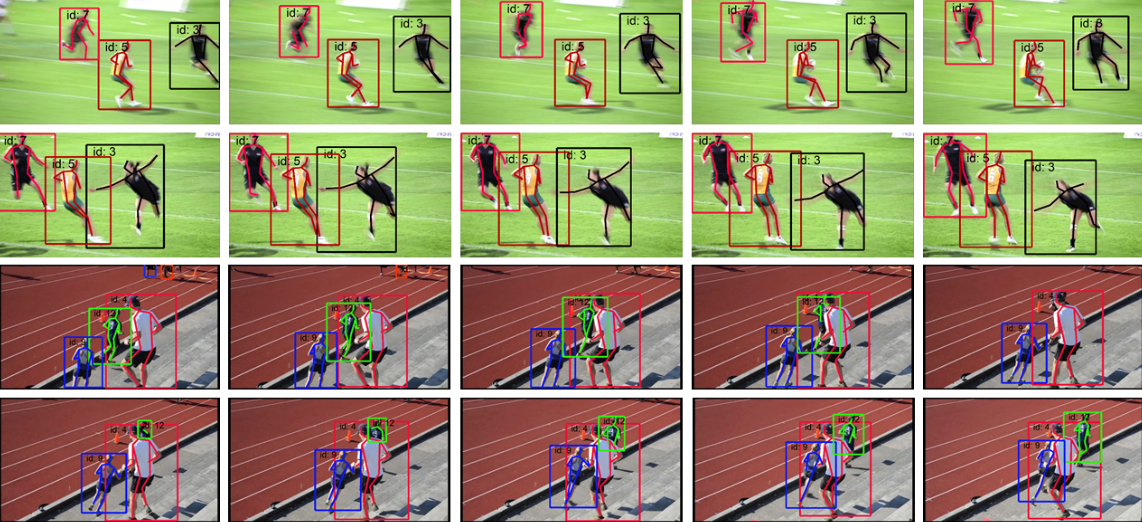
\includegraphics[width=0.5\textwidth]{figures/sample.png}
            \caption{Some sample results on PoseTrack Challenge test set}
        \end{figure}

        This approach's simplicity is one of its main advantages. This work shows that a straightforward approach may still provide outstanding results, even in the face of the growing complexity of algorithms and systems in this sector. For the purpose of developing and assessing new techniques, this simplifies the process of analysing and comparing algorithms. It can be concluded that Simple Baselines for Human Pose Estimation and Tracking offers a productive and successful method for these tasks. Its ease of use and potency make it a useful instrument in its field, and there is a lot of room for expansion.

    \subsection{Pose2Seg: Detection Free Human Instance Segmentation \parencite{zhang2019pose2segdetectionfreehuman}}
        Pose2Seg, created by Song-Hai Zhang et al., is an innovative approach to human instance segmentation. This method provides a unique posture-based instance segmentation framework for humans, which divides instances based on human position, as opposed to proposal region identification. Usually, image instance segmentation begins with object detection and proceeds to segment the object from the detection bounding-box. Conversely, Pose2Seg takes into account the uniqueness of the ``human'' category, which is precisely specified by the posture skeleton. The human posture skeleton may be used to identify instances with severe occlusion instead of bounding-boxes.\\
        
        \begin{figure}[htbp]
            \centering
            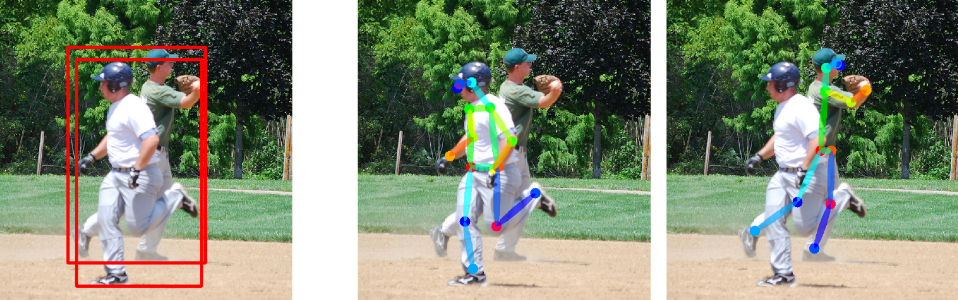
\includegraphics[width=0.5\textwidth]{figures/Pose2Seg.png}
            \caption{Heavily occluded people are better separated using human pose than using bounding-box.}
        \end{figure}

        This method shows that the pose-based framework can better handle occlusion and obtain higher accuracy on the human instance segmentation test compared to the most sophisticated detection-based approach. Additionally, the publication ``Occluded Human (OCHuman)'' introduces a new benchmark for occluded persons with full annotations, including instance masks, bounding boxes, and human position. This dataset has 8110 meticulously annotated human occurrences dispersed throughout 4731 images. All things considered, Pose2Seg offers a fresh and effective method for segmenting human instances. Its detection-free segmentation based on human postural capability makes it a top tool in its field with a lot of future application possibilities. 
    \subsubsection{Summary}
        The science of human posture evaluation has greatly benefited from these four publications. BlazePose makes real-time body location tracking of mobile devices easy and effective. To illustrate the effectiveness of nonparametric representations in the precise estimation of multi-person poses, Realtime Multi-Person 2D Pose Estimation uses component affinity fields. The realistic baseline techniques for posture estimation and tracking provided by Simple Baselines for Human posture Estimation and Tracking emphasise the importance of simplicity in obtaining high performance. Pose2Seg offers a unique pose-based instance segmentation framework and is the last illustration of the potential for detection-free human instance segmentation. By building on the concepts of others, proposing fresh ideas, and refining previously established methods, each study advances the subject of human pose assessment.



\section{Research Methods} % ~250 words
% Briefly discuss the research methods that may be appropriate for the proposed research. For example, are they quantitative or qualitative and how would you deploy them? Will you use any publicly available data?
    This research project will attempt to provide a framework for performing physical interventions that enhance the physical well-being of patient populations and to extract skeleton-based features that can quantify the physical status of each user. To avoid ethical concerns, there will be no data collection or participant enrollment in this research project. This research will involve the process of analysing numerical data from video frames. This numerical data will refer to the coordinates of the key points and which keypoints are linked. Therefore, this research is quantitative.\\
    This research will act as a study about the creation of an application which provides a framework for sports professionals to set their desired ranges of motion and form constraints on specific exercises to create personalised workout regimens.  \\
    The extracted video markers will be analysed to determine the efficacy and accuracy of the pose estimation techniques used. Each individual exercise type will require its own model trained for that specific movement. Video markers will be extracted from recording I will take of myself and the ones provided by my supervisor to evaluate pose estimation accuracy.\\
    The expected outcome is to have many models capable of detecting the user's poses and extracting useful and relevant data for sports professionals, regular gym goers, and home workout enjoyers to understand and use.





\section{Ethical Considerations} % ~250 words
% In consultation with your supervisor, you must evidence any ethical issues in this section and clearly identify if you have submitted an ethical application via LEAS.
    After careful consideration, my supervisor and I have decided to avoid the need to submit an ethical application by not collecting any data ourselves or involving any external human participation. All the data used will be either given to me by my supervisor or produced by myself for testing and validation procedures only.

\section{Project Plan and Risk Analysis} % ~300 words 
% A documented project plan spanning the full timeframe of the project. Timescales and milestones/deliverables should be provided for each of the project objectives. This may take the form of a Gantt chart, with granularity of no more than one week. The risk analysis should identify and explain specific risks, their likelihood, and assessed impact, with a mitigation strategy for each. Generic risks (e.g., illness, loss of data, IT problems etc.) are common to all projects and should NOT be included here.
    \subsection{Project Plan}
        Figure~\ref{fig:gantt} is a gantt chart showing the phases of work I will be attempting to follow over the course of this project. The two greyed out bars are periods where I will be unable to work on this project as I'll be travalling on AgriFoRwArdS CDT duties. There are three major milestones for this project, the submission date for this proposal on the 4th of July, the sumbmission date for this projecton the 29th of August, and the in person viva defence of the MSc on the week of the 16th of September.
        \begin{figure}[htbp]
            \centering
            \begin{sideways}
                \begin{ganttchart}[y unit title=0.4cm,
                    y unit chart=0.5cm,
                    x unit = 0.2cm,
                    vgrid,hgrid, 
                    title label anchor/.style={below=-1.6ex},
                    % title label font=\tiny,
                    title left shift=.05,
                    title right shift=-.05,
                    title height=1,
                    progress label text={},
                    bar height=0.7,
                    group right shift=0,
                    group top shift=.6,
                    group height=.3]{1}{84}

                    %labels
                    \gantttitle{July}{31}
                    \gantttitle{August}{31} 
                    \gantttitle{September}{22} \\
                    
                    \gantttitle{week 1}{7}
                    \gantttitle{week 2}{7}
                    \gantttitle{week 3}{7}
                    \gantttitle{week 4}{7}
                    \gantttitle{week 5}{7}
                    \gantttitle{week 6}{7}
                    \gantttitle{week 7}{7}
                    \gantttitle{week 8}{7}
                    \gantttitle{week 9}{7}
                    \gantttitle{week 10}{7}
                    \gantttitle{week 11}{7}
                    \gantttitle{week 12}{7}\\


                    %tasks
                    \ganttbar[progress=0]{CDT Summer School}{7}{13} \\    %elem0
                    \ganttbar[progress=0]{CDT Annual Conference}{22}{23}\\%elem1
                    \ganttbar{Proposal Writing}{1}{3} \\%elem2
                    \ganttmilestone{Proposal submission}{4}\\%elem3
                    \ganttbar{Code (Feature extraction)}{5}{6}\\%elem4
                    \ganttbar{Code (Preprocessing)}{14}{21}\\%elem5
                    \ganttbar{Testing}{19}{21}\\%elem6
                    \ganttmilestone{First system version}{21}\\%elem7
                    \ganttbar{Code (AI algorithms)}{24}{53}\\%elem8
                    \ganttbar{Testing}{40}{53}\\%elem9
                    \ganttmilestone{Final sytem version}{53}\\%elem10
                    \ganttbar{Paper Writing}{38}{59}\\%elem11
                    \ganttmilestone{Sumbission Deadline}{60}\\%elem12
                    \ganttbar{Presentation planning}{62}{69}\\%elem13
                    \ganttbar{Viva Preparation}{67}{77}\\%elem14
                    \ganttmilestone{In Person Viva}{78}%elem15

                    
                    %relations 
                    \ganttlink{elem2}{elem3}
                    \ganttlink{elem4}{elem5}
                    \ganttlink[link type=dr]{elem5}{elem6}
                    % \ganttlink{elem5}{elem7}
                    \ganttlink[link type=dr]{elem6}{elem7}
                    \ganttlink{elem7}{elem8}
                    \ganttlink[link type=dr]{elem8}{elem9}
                    % \ganttlink{elem8}{elem10}
                    \ganttlink{elem9}{elem10}
                    \ganttlink{elem11}{elem12}
                    \ganttlink[link type=dr]{elem13}{elem14}
                    \ganttlink{elem14}{elem15}

                \end{ganttchart}
            \end{sideways}
        \caption{Gantt Chart}~\label{fig:gantt}
        \end{figure}
    \subsection{Risk Analysis}
        \begin{table}[htbp]
            \centering
            \resizebox{\columnwidth}{!}{%
            \begin{tabular}{|c|c|c|c|c|l}
            \cline{1-5}
            ID &
            Description &
            Impact &
            Likelihood &
            \begin{tabular}[c]{@{}c@{}}mitigation \\ strategy\end{tabular} &
            \\ \cline{1-5}
            R1 &
            \begin{tabular}[c]{@{}c@{}}A progam\\ doesn't work or is\\ incompatable with my\\ machine\end{tabular} &
            high &
            medium &
            \begin{tabular}[c]{@{}c@{}}find a alternative\\ program\end{tabular} &
            \\ \cline{1-5}
            R2 &
            \begin{tabular}[c]{@{}c@{}}The landmark detection\\ doesn't function for \\ everyone\end{tabular} &
            low &
            medium &
            \begin{tabular}[c]{@{}c@{}}We won't be able\\ to know if that is\\ the case\end{tabular} &
            \\ \cline{1-5}
            R3 &
            \begin{tabular}[c]{@{}c@{}}Too much data is created\\ for my computer to store\end{tabular} &
            high &
            low &
            \begin{tabular}[c]{@{}c@{}}Reduce the amount\\ of data and make \\ smaller models\end{tabular} &
            \\ \cline{1-5}
            R4 &
            \begin{tabular}[c]{@{}c@{}}The movement detections\\ are slow which cause them\\ to be inaccurate\end{tabular} &
            high &
            medium &
            \begin{tabular}[c]{@{}c@{}}Reduce the amount\\ of keypoints to detect\\ to the strictly necessairy\\ ones\end{tabular} &
            \\ \cline{1-5}
            \end{tabular}%
            }
            \caption{Table describing the potential risks, how severe they are, how likely they are, and what to do if they occur}~\label{tab:risk}
        \end{table}

    
\newpage
\printbibliography%
\centering{\large{\textbf{Word Count: 2522}}}
\end{document}
